\documentclass[12pt]{exam}
\usepackage[utf8]{inputenc}

\usepackage[margin=.5in]{geometry}
\usepackage{amsmath,amssymb}
\usepackage{multicol}
\usepackage{datetime}
\usepackage{graphicx}
\graphicspath{ {./images/} }

\usepackage{tikz}
\usetikzlibrary{graphs,arrows.meta}


\pagestyle{head}
\firstpageheader{}{}{}
\runningheader{\class}{\examnum\ - Page \thepage\ of \numpages}{\examdate}
\runningheadrule

\newcommand{\class}{3013 - Algorithms}
\newcommand{\term}{Spring 2020}
\newcommand{\examnum}{Final Exam}
\newcommand{\examdate}{\today}
\newcommand{\timelimit}{None}
\newcommand{\seperate}{\begin{center}\noindent\rule{18cm}{0.75pt}\end{center}}

\begin{document}

\noindent
\begin{tabular*}{\textwidth}{l @{\extracolsep{\fill}} r @{\extracolsep{6pt}} l}
    \textbf{\class} & \textbf{Name:} & \makebox[2in]{\hrulefill}\\
    \textbf{\term} &&\\
    \textbf{\examnum} &&\\
    \textbf{\examdate} &&\\
    % \textbf{Time Limit: \timelimit} & Teaching Assistant & \makebox[2in]{\hrulefill}
\end{tabular*}\\

\rule[2ex]{\textwidth}{2pt}

\renewcommand{\arraystretch}{1.25}
\begin{tabular}{ | p{16cm} | }
    \hline
    \textbf{READ THESE INSTRUCTIONS}\\
    \hline
\begin{itemize}
  \item Create a digital document that has zero handwriting on it
  \item Questions should be answered in order and clearly marked.
  \item Your name should be on each page, in the heading if possible.
  \item Turn your final in by uploading to D2L. Link should be obvious.
\end{itemize}

    \hline
    \textbf{Failure to comply will result in loss of letter grade.}\\
    \hline
    This exam is \numpages\ pages (without cover page) and \numquestions\ questions. Total of points is \numpoints.\\
\end{tabular}
\begin{center}

    Grade Table (don't write on it)\\
    \addpoints
    \gradetable[v][questions]
\end{center}

\noindent
\rule[2ex]{\textwidth}{2pt}
\clearpage



\begin{questions}
    \question[15] Problem solving paradigms.
    \begin{parts}
        \part List the 4 problem solving paradigms.
        \part Give 2 example algorithms that fit into each paradigm

    \end{parts}


    %######################
    \seperate
    %######################

    \question[20]List the complexities from fastest to slowest.

    \begin{tabular}{ c  c  c  c  c  c  c  c c }
        \multicolumn{8}{c}{Complexity Choices} \\
        $O(n!)$ & $O(2^n)$ & $O(1)$ & $O(n\ lg\ n)$ & $O(n^2)$ & $O(n^n)$ & $O(n)$ & $O(log\ n)$ & None of These \\
    \end{tabular}


    %######################
    \seperate
    %######################

    \question[20] Given the following binary tree:

    \includegraphics[scale=.35]{graphics/tree_again.png}

    \begin{enumerate}
        \item What is the height of this tree?
        \item What is the root of this tree?
        \item How many leaves does this tree have? List them.
        \item How many descendants does 23 have?
        \item How many siblings does 23 have?
        \item Who is the predecessor of 23?
        \item Who is the successor of 23?
    \end{enumerate}

    %######################
    \seperate
    %######################

    \question[20]Assign the correct complexity to each item below.

    \begin{tabular}{ c  c  c  c  c  c  c  c c }
        \multicolumn{8}{c}{Complexity Choices} \\
        $O(n!)$ & $O(2^n)$ & $O(1)$ & $O(n\ lg\ n)$ & $O(n^2)$ & $O(n^n)$ & $O(n)$ & $O(log\ n)$ & None of These \\
    \end{tabular}
    \\
    \renewcommand{\theenumi}{\Alph{enumi}}
    \begin{enumerate}
        \item $\rule{2cm}{0.15mm}$ Inserting an element into a balanced binary search tree.
        \item $\rule{2cm}{0.15mm}$ Finding an element in a list.
        \item $\rule{2cm}{0.15mm}$ Finding an element in an ordered list.
        \item $\rule{2cm}{0.15mm}$ Removing an element from a binary heap.
        \item $\rule{2cm}{0.15mm}$ Finding an element in a binary search tree.
        \item $\rule{2cm}{0.15mm}$ Adding an element to a binary heap.
        \item $\rule{2cm}{0.15mm}$ Building a binary heap given an array of values.
        \item $\rule{2cm}{0.15mm}$ Building a binary heap given a linked list of values.
        \item $\rule{2cm}{0.15mm}$ Remove an item from a linked list of values.
        \item $\rule{2cm}{0.15mm}$ Insert an item into an ordered linked list of values.
    \end{enumerate}

    \seperate

    \question[10] \textbf{Heapify}: Describe what it does, and why it is significant. Be thorough.


    %######################
    \seperate
    %######################

    \question[15] Write a pseudo code implementation for deleting a node from a binary search tree.

    %######################
    \seperate
    %######################

    \question[10] Take the values from the max heap below and draw an array that would represent this tree.

    Put the answer on your answer sheet using something similar to:  \includegraphics[scale=.35]{graphics/empty_array.png}

    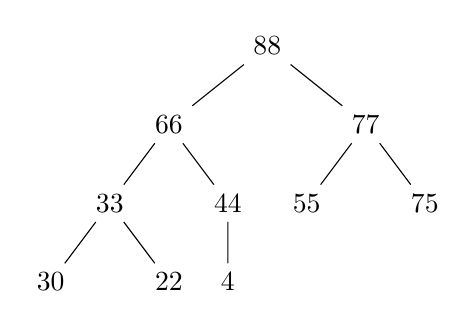
\begin{tikzpicture}[level distance=1cm,
            level 1/.style={sibling distance=2.5cm},
            level 2/.style={sibling distance=1.5cm}]
        \node {88}
        child {node {66}
                child {node {33}
                        child {node {30}}
                        child {node {22}}
                    }
                child {node {44}
                        child {node {4}}
                    }
            }
        child {node {77}
                child {node {55}}
                child {node {75}}
            };
    \end{tikzpicture}

    %######################
    \seperate
    %######################

    \question[15] Given a sequence of numbers: 19, 6, 8, 11, 4, 5
    \begin{parts}
        \part Draw a binary min-heap (in a tree form) by inserting the above numbers reading them from left to right
        \part Show a tree that can be the result after the call to deleteMin() on the above heap
        \part Show a tree after another call to deleteMin()
    \end{parts}

    %######################
    \seperate
    %######################


    \question[30] List vs Array based data structures. Given a statement below, choose:\\
    \textbf{List}, \textbf{Array}, \textbf{Both}, \textbf{None}\\
    to indicate what the statement is implying.

    \begin{tabular}{ c  c  c  c }
        \textbf{Choices:} List & Array & Both & None \\
    \end{tabular}

    \renewcommand{\theenumi}{\Alph{enumi}}
    \begin{enumerate}
        \item Directly access element in this structure.
        \item Bounded by size.
        \item Easy to insert and delete from.
        \item Easy to implement.
        \item More overhead.
        \item Can be sorted.
        \item Must be allocated in the heap.
        \item Expensive to resize.
        \item Grows and shrinks easily.
        \item Binary search can be performed on this.
        \item Easily access each element in this structure.
        \item Cannot be allocated in the heap.
        \item Must be statically declared.
        \item Items added to front or rear.
        \item Easier to delete from middle.
        \item Can be used to represent a binary tree.
    \end{enumerate}


    \question[15] Give a pre-order / post-order /in-order traversal of the following tree:

    \includegraphics[scale=.5]{graphics/tree_traverse.png}

    \question  Stack based memory VS Heap based memory.
    \begin{parts}
        \part[10]Pros and cons of a Stack
        \part[10]Pros and cons of the Heap
    \end{parts}

    \question
    \begin{parts}
        \part[10] Draw the resulting binary search tree by inserting the following values from left to right: \textbf{19, 6, 8, 11, 4, 13, 5, 27, 43, 49, 31, 25}
        \part[10] Delete \textbf{19} from the binary search tree in part (a) using a standard removal algorithm for binary search trees. Draw the TWO potential binary search trees that you can end up with.
    \end{parts}

    %######################
    \seperate
    %######################

    \question[20] You are attending a party with $n$ other people. Each other person $i$ arrives at the party at some time
    $s_i$ and leaves the party at some time $t_i$ (where $s_i < t_i$). Once a person leaves the party, they do not return.
    Additionally, each person $i$ has some coolness $c_i$. At all times during the party, you choose to talk to the coolest person currently at the party. (All coolness values are distinct.) If you are talking to someone, and someone else cooler arrives at the party, you leave your current conversation partner and talk to the new person. If the person you are talking to leaves the party, you go talk to the coolest person remaining at the party. (This might or might not be a person with whom you have already talked.) You are the first to arrive at the party and the last to leave. Additionally, you are the most popular
    person at the party, so everyone wants to talk with you.

    Describe a data structure which allows you to decide in $O(1)$ time to whom you should talk at any moment. You should be able to update this data structure in $O(log n)$ time when someone arrives or leaves.

    \question[5]Write your name on your answer sheets.

\end{questions}
\end{document}